%
% ---------------------------------------------------
%
% Proyecto de Final de Carrera:
% Author: José Lucas Grillo Lorenzo <jlucas.gl@gmail.com>
% Capítulo: Resultados computacionales 
% Fichero: Cap7_resultados.tex
%
% ----------------------------------------------------
%

\chapter{Resultados computacionales} \label{chap:resultados}  

En este Capítulo se presentan una serie de resultados evaluando
diversos tests compilados con \accULL{}, y algunos de los compiladores comerciales de 
\OpenACC{} disponibles en el mercado. En él se detalla en qué consisten 
dichos tests y la infraestructura hardware sobre la que se han realizado los experimentos,
así como una comparativa del rendimiento alcanzado con los mismos.
Se describirán posteriormente los tests sobre los que se ha trabajado. 
Concretamente, tres experimentos del conjunto de pruebas \rodinia{} 
\cite{URL::Rodinia}, un código de multiplicación de matrices, y el \benchmark{} para 
\OpenACC{} del \epcc{} publicado recientemente 
en su web \cite{URL::ACCepccB}. Aportando medidas de rendimiento en aceleración o tiempo 
de compilación cuando se dispongan.

\section{Plataforma hardware}

A continuación se describe las características de la plataforma hardware sobre la que
han realizado las pruebas de experimentación:

\begin{itemize}
	\item \texttt{Garoe}: Una \textit{Workstation} con un procesador \textbf{Intel Core i7 930} a 2.80 GHz con 1MB de cache L2 y 8MB de cache L3 compartida por los cuatro núcleos. Este computador tiene 4 GB de memoria RAM y dos \GPU{}'s de \NVIDIA{} conectadas a este sistema: una Tesla M2090 con 512 núcleos CUDA y 5GB de memoria (Fermi), y una Tesla K20c
	con 2496 núcleos CUDA y 4GB de memoria (Kepler).
En este servidor se han realizado las pruebas con los \benchmark{}s de \rodinia{}.
	\item \texttt{Verode}: Un \textit{cluster} que contiene procesadores de dos \textit{quad core} \textbf{Intel Xeon E5410} a 2.25GHz, 24GB de memoria y una \GPU{} Fermi C2050 con 4GB de memoria en el nodo \textit{verode16}. El nodo de compilación \textit{verode00} es virtualizado. En \texttt{Verode} se ha evaluado el rendimiento de \accULL{} con la \epcc{} \OpenACC{} \benchmark{} suite.
\end{itemize}

Con la plataforma \texttt{Garoe} se pretende simular un escenario habitual para un 
desarrollador de \OpenACC{}, es decir, un usuario con cierta experiencia 
interesado en mejorar el rendimiento de un código, podría adquirir una \GPU{} e insertarla
en su sobremesa. Es una solución relativamente barata, a cambio de un incremento
considerable en el rendimiento con muy poco esfuerzo de desarrollo.

En el otro extremo se encuentra \texttt{Verode16}, un nodo de un \textit{cluster}
heterogéneo de alto rendimiento. Los \textit{cluster}s heterogéneos son frecuentes
en los centros de supercomputación de hoy en día. Al estar compuestos por 
sistemas multinúcleo y aceleradores gráficos, se facilita el uso de \OpenACC{} en estas 
plataformas. 

\section{Software evaluado}

En los experimentos realizados se han evaluado tres compiladores con soporte para 
\OpenACC{}. Para el conjunto de tests de la suite \epcc{} \OpenACC{} \benchmark{} se han 
empleado los últimos compiladores disponibles hasta la fecha. En el caso de los resultados 
de los tests \rodinia{} medidos en Garoe se incluyen resultados obtenidos con versiones anteriores de los
compiladores por tener una referencia comparativa.
A continuación se muestra una descripción de los compiladores empleados en cada caso:

\begin{itemize}
\item \PGI{} OpenACC en su versión 12.5 para el \benchmark{} \rodinia{} y la multiplicación de matrices (MxM), usando la versión 13.5 (la más reciente hasta la fecha) para la suite \epcc{} \OpenACC{} \benchmark{}. 
\item \CAPS{} HMPP con soporte para \OpenACC{}, versión 3.3.3 para la suite \epcc{} \OpenACC{}, y la versión 3.3.1 para los tests \rodinia{} y MxM. 
\item \accULL{} versión 0.1b para \rodinia{} \benchmark{} suite y MxM, mientras que  para la suite \epcc{} \OpenACC{} \benchmark{} se ha empleado la versión 0.3alpha.
\end{itemize}

\section{Rodinia \benchmark{} suite}

El conjunto de pruebas \rodinia{} \cite{Che:2010:CRB} está compuesto de 
programas de cómputo intensivo diseñados para ser ejecutados en entornos 
masivamente paralelos como los de una \GPU{}, cubriendo un amplio rango de 
aplicaciones.
La suite incluye versiones para la mayoría de los códigos en OpenMP, CUDA y OpenCL,
demostrando la viabilidad de la programación basada en directivas y su facilidad de uso.
En esta Sección se
presenta el rendimiento para tres \benchmark{}s extraídos de la suite. Dichos 
\benchmark{}s han sido anotados con 
\OpenACC{} a partir de la versión \OpenMP{} con relativa facilidad.
En esta contribución se proporcionan los resultados computacionales de tres códigos:
una descomposición LU (\texttt{LUD}),
una herramienta de simulación térmica (\texttt{HS}) y un método de optimización global 
no lineal para alineamientos de secuencias de ADN (\texttt{NW}).
En las Tablas \ref{table:rodinia:fermi} y \ref{table:rodinia:kepler} se muestra una 
comparativa de rendimiento entre dos \GPU{}s con arquitectura Fermi y Kepler 
respectivamente, 
con las implementación \OpenACC{} usando los compiladores de \PGI{}, \CAPS{} y \accULL{}, 
respecto a la implementación con \CUDA{} nativo.

\subsection{HotSpot (\texttt{HS})}

HotSpot (\texttt{HS}) es una herramienta de simulación térmica usada para
estimar la temperatura del procesador basada en un superficie plana y medidas de 
disipación de potencia simuladas.

La implementación de \rodinia{} incluye el kernel 2D de simulación térmica transitoria
de \texttt{HS},
que calcula iterativamente una serie de ecuaciones diferenciales para bloques de 
temperatura. 
Las entradas al programa son la potencia y las temperaturas iniciales. 
Cada celda de salida de la malla representa el valor de temperatura media del área
correspondiente del chip.

%%%%%%%%%%%%%%%%%%%%%%%%%%%%%%%%%%%%%%%%%%%%%%%%%%%%%%%%%%%%%%
\begin{lstlisting}[caption={Bucle principal de \texttt{HS}},label=code:HS]
for (i = 0; i < num_iterations ; i++) { 
    /* Compute current temperatures */
    for (r = 0; r < row; r++) 
      for (c = 0; c < col; c++) 
          ...
    /* Update */
    for (r = 0; r < row; r++) 
      for (c = 0; c < col; c++) 
          ...
  }
\end{lstlisting}
%	%%%%%%%%%%%%%%%%%%%%%%%%%%%%%%%%%%%%%%%%%%%%%%%%%%%%%%%%%%%%%
El Listado \ref{code:HS} muestra una versión resumida de la rutina principal de
 \texttt{HS}. Contiene dos bucles anidados que se ejecutan durante un número determinado 
de iteraciones. El primer bucle computa la temperatura actual de cada posición dentro del 
chip, mientras que el segundo, solo actualiza los datos con la información calculada en la 
iteración actual.

%%%%%%%%%%%%%%%%%%%%%%%%%%%%%%%%%%%%%%%%%%%%%%%%%%%%%%%%%%%%%%
\begin{lstlisting}[caption={Boceto de \texttt{HS} usando \OpenACC{}},label=code:HS:openacc]
void do_iteration(double * temp,...) {
 #pragma acc kernels ....
   { /* Compute current temperatures */
     #pragma acc loop ... 
     for (r = 0; r < row; r++) 
       for (c = 0; c < col; c++) 
           ...
     /* Update */
     #pragma acc loop ...
     for (r = 0; r < row; r++) 
         for (c = 0; c < col; c++) 
              ....
   }
}
void routine(...) {
...
#pragma acc data copy(temp,...)
for (i = 0; i < n_it ; i++)
    do_iteration(temp ... )
}
\end{lstlisting}
%%%%%%%%%%%%%%%%%%%%%%%%%%%%%%%%%%%%%%%%%%%%%%%%%%%%%%%%%%%%%%

En el Listado \ref{code:HS:openacc} se muestra un boceto del código del Listado 
\ref{code:HS}, etiquetado con directivas \OpenACC{}. Como se puede apreciar,
es necesario cargar en el dispositivo las variables de entrada como \texttt{temp}. Esto
se logra con \texttt{\#pragma acc data copy(temp,..)} englobando la región del
código que ha de ser tratado por la \gpu{} en la función \method{routine}. Una vez 
cargadas las variables de entrada en el acelerador, mediante \texttt{\#pragma acc kernels} 
y haciendo uso de las cláusulas \texttt{loop} se construye el segmento de código del 
kernel que será ejecutado en el dispositivo. 

Tanto en la Figura \ref{fig:allfermi} como en la \ref{fig:allkepler} se puede observar el buen 
rendimiento alcanzado
con este código, respecto a las implementaciones alcanzadas con otros compiladores. No 
obstante es de esperar que en versiones más recientes de los compiladores analizados 
esta diferencia sea menor. Pese a esto, los trabajos abordados en la versión 0.3alpha de 
\accULL{} en materia de optimizaciones de bucles resuelven buena parte de las carencias de 
las versiones anteriores.

%%%%%%%%%%%%%%%%%%%% Fig. %%%%%%%%%%%%%%%%%%%%%%%%%%%%%%%%%%%
\begin{figure}[t]
\centering
\includegraphics[width=\linewidth]{resultados/2_fermi_Computing.png}
\caption{Aceleración relativa a la implementación nativa en \CUDA{} para los códigos \texttt{MxM}, \texttt{LUD}, \texttt{HS} y \texttt{NW} la \GPU{} Fermi}
\label{fig:allfermi}
\end{figure}
%%%%%%%%%%%%%%%%%%%%%%%%%%%%%%%%%%%%%%%%%%%%%%%%%%%%%%%%%%%%%


%%%%%%%%%%%%%%%%%%%% Fig. %%%%%%%%%%%%%%%%%%%%%%%%%%%%%%%%%%%
\begin{figure}[t]
\centering
\includegraphics[width=\linewidth]{resultados/3_kepler_Computing.png}
\caption{Aceleración relativa a la implementación nativa en \CUDA{} para los códigos \texttt{MxM}, \texttt{LUD}, \texttt{HS} y \texttt{NW} un la \GPU{} Kepler}
\label{fig:allkepler}
\end{figure}
%%%%%%%%%%%%%%%%%%%%%%%%%%%%%%%%%%%%%%%%%%%%%%%%%%%%%%%%%%%%%

\subsection{Needleman-Wunsch (\texttt{NW})}

Needleman-Wunsch (\texttt{NW}) es un método de optimización global no lineal para 
el alineamiento de secuencias de ADN.
Los potenciales pares de secuencias se organizan en una matriz 2D. 
En el primer paso, el algoritmo rellena la matriz desde la esquina superior izquierda 
hasta la esquina inferior derecha, paso a paso.
El alineamiento óptimo es un camino que tiene una puntuación máxima, siendo esta 
puntuación el valor del camino más pesado que termina en ese elemento.
Así, el valor de cada elemento depende de sus elementos vecinos más cercanos al norte, 
noroeste y oeste. En el segundo paso, el camino máximo es recorrido a la inversa para 
deducir el alineamiento óptimo. Aplicar la planificación adecuada a las iteraciones del 
bucle, es crítico para mejorar el rendimiento.

En este caso, se puede apreciar en la Figura \ref{fig:allfermi} y \ref{fig:allkepler} que 
el mapeo que usa la implementación de \CAPS{} \OpenACC{} es bastante buena, dando
como resultado un rendimiento razonablemente bueno. Se ha experimentado con diferentes
valores de la cláusula \gang{} para alcanzar el mejor rendimiento posible, al igual
que se hizo con la implementación con \PGI{}.
El rendimiento de la implementación con \PGI{} es el peor en este caso. Esto es debido, a 
que pese al esfuerzo para forzar al compilador a volcar los bucles a la \gpu{}, su 
análisis de dependencias creó kernels secuenciales en \GPU{}. Gracias a la información
volcada en tiempo de compilación ha sido posible detectar que la implementación \accULL{} 
ha podido paralelizar las falsas dependencias entre iteraciones. Lo que redunda en el
buen rendimiento alcanzado, respecto a la versión nativa de \CUDA{}, y en general en comparación con el resto de compiladores evaluados.

\subsection{Descomposición LU (\texttt{LUD})}

La descomposición LU (\texttt{LUD}) es un algoritmo bien conocido
para calcular las soluciones de un conjunto lineal de ecuaciones.
El kernel \texttt{LUD} descompone una matriz como producto de una matriz triangular
inferior y una matriz triangular superior. Esta aplicación tiene muchas dependencias 
entre filas y columnas, y exige algunas optimizaciones importantes para alcanzar
un buen rendimiento paralelo.
En las Tablas \ref{table:rodinia:fermi} y \ref{table:rodinia:kepler} se muestra, 
para la tarjeta Fermi y para la Kepler respectivamente, la aceleración respecto 
a la implementación nativa con CUDA de este algoritmo.

Aunque en este caso el mejor rendimiento se alcanza para tamaños pequeños, es importante
destacar el excepcional rendimiento alcanzado con tamaños grandes en la implementación
nativa. Sin embargo, la complejidad de las dependencias dentro del bucle, dificultan 
enormemente la implementación usando directivas.
La implementación nativa usa ampliamente la memoria compartida, que no usa actualmente 
\accULL{}. El compilador de \PGI{} cachea algunos arrays en memoria compartida, logrando 
así un rendimiento superior al de \accULL{} en este problema. Un caso similar ocurre con el 
compilador de \CAPS{} sobre \OpenACC{}.

%%%%%%%%%%%%%%%%%%%%% Table %%%%%%%%%%%%%%%%%%%%%%%%%%%%%%%%%
\begin{table}[htb]
\caption{Aceleración relativa a CUDA nativo %($t_{CUDA} / t$) 
		para distintos tamaños del problema con 
         \texttt{LUD}, \texttt{HS} y \texttt{NW} usando la GPU Fermi.}
\label{table:rodinia:fermi}
\newcommand{\m}{\hphantom{$-$}}
%\newcommand{\cc}[1]{\multicolumn{1}{c}{#1}}
\renewcommand{\tabcolsep}{4pt} % enlarge column spacing
\renewcommand{\arraystretch}{1.2} % enlarge line spacing
\centering
\begin{tabular}{@{}ccccc}
\hline 
       & Tamaño & PGI & CAPS    & \accULL{} \\
\hline
\multirow{2}{*}{HS}  
      &   512  &  0.164      &  0.184  &  0.562    \\
      &  1024  &  0.323      &  0.426  &  0.506    \\
\hline
\multirow{2}{*}{NW}  
      &  2048  &  0.079      &  0.678  &  0.696    \\ 
      &  4096  &  0.073      &  0.495  &  0.552    \\
\hline
\multirow{3}{*}{LUD}  
      &   512  &  0.349      &  2.230  &  0.104    \\
      &  1024  &  0.065      &  0.270  &  0.010    \\
      &  2048  &  0.035      &  0.100  &  0.002    \\
\hline
\end{tabular}\\[2pt]
\end{table}
%%%%%%%%%%%%%%%%%%%%%%%%%%%%%%%%%%%%%%%%%%%%%%%%%%%%%%%%%%%%%%

%%%%%%%%%%%%%%%%%%%%% Table %%%%%%%%%%%%%%%%%%%%%%%%%%%%%%%%%
\begin{table}[htb]
\caption{Aceleración relativa a CUDA nativo ($t_{CUDA} / t$) 
		para distintos tamaños del problema con 
         \texttt{LUD}, \texttt{HS} y \texttt{NW} usando la GPU Kepler.}
\label{table:rodinia:kepler}
\newcommand{\m}{\hphantom{$-$}}
%\newcommand{\cc}[1]{\multicolumn{1}{c}{#1}}
\renewcommand{\tabcolsep}{4pt} % enlarge column spacing
\renewcommand{\arraystretch}{1.2} % enlarge line spacing
\centering
\begin{tabular}{@{}ccccc}
\hline 
       & Tamaño & PGI & CAPS    & \accULL{} \\
\hline
\multirow{2}{*}{HS}  
       &  512  &  0.278      &  0.300  &  1.070    \\
       & 1024  &  0.312      &  0.351  &  0.723    \\
\hline
\multirow{3}{*}{NW}  
       & 2048  &  0.251      &  2.343  &  2.439    \\ 
       & 4096  &  0.137      &  1.035  &  0.951    \\
       & 8192  &  0.116      &  0.653  &  0.709    \\
\hline
\multirow{3}{*}{LUD}  
       &  512  &  0.570      &  3.192  &  0.192    \\
       & 1024  &  0.217      &  0.795  &  0.032    \\
       & 2048  &  0.091      &  0.185  &  0.005    \\
\hline
\end{tabular}\\[2pt]
\end{table}
%%%%%%%%%%%%%%%%%%%%%%%%%%%%%%%%%%%%%%%%%%%%%%%%%%%%%%%%%%%%%%

\section{Multiplicación de matrices}

La multiplicación de matrices (\texttt{MxM}) es un \textit{kernel} muy usado para mostrar 
el rendimiento pico de una GPU. La versión del producto de matrices que hemos utilizado se 
centra en el algoritmo de multiplicación por bloques, similar al que se usa en las 
librerías BLAS \cite{Dongarra:1990:ASL}.

El Listado \ref{code:mxm} muestra el código de \texttt{MxM} por bloques anotado con 
OpenACC. Este es el código tal como debía ser rediseñado en la versión 0.1b de \accULL{}.
Para este código se ha usado la directiva \texttt{kernels}. Esta directiva crea una 
región de datos y un conjunto de variables que son copiadas al interior de la región. 
Dentro de la región \texttt{kernels} se definen dos bucles que el compilador 
\texttt{accULL} descargará hacia la GPU mediante un \textit{kernel}. El primer bucle 
(línea 4)  inicializa la matriz. La cláusula \texttt{collapse} de la línea 3 indica al 
compilador que para el bucle que le sigue se cree un \textit{kernel} con una estructura 
2D. %% CONFIRMAR !!
En la línea 12 se vuelve a hacer uso de la cláusula \texttt{collapse}, y 
\texttt{accULL} genera otro \textit{kernel} 2D que iterará sobre los bloques de la matriz. 

%%%%%%%%%%%%%%%%%%%% Code  %%%%%%%%%%%%%%%%%%%%%%%%%%%%%%%%%%%
\begin{lstlisting}[caption={\texttt{MxM} por bloques en OpenACC},label=code:mxm]
#pragma acc kernels name("mxm") copy(a[L*N]) copyin(b[L*M],c[M*N]) 
{
#pragma acc loop private(i, j) collapse(2)
for (i = 0; i < L; i++)
  for (j = 0; j < N; j++)
    a[i * L + j] = 0.0;
/* Iterate over blocks */
for (ii = 0; ii < L; ii += tile_size)
 for (jj = 0; jj < N; jj += tile_size)
  for (kk = 0; kk < M; kk += tile_size) {
   /* Iterate inside a block */
   #pragma acc loop collapse(2) private(i,j,k)
   for (j=jj; j < min(N, jj+tile_size); j++) 
    for (i=ii; i < min(L, ii+tile_size); i++)
     for (k=kk; k < min(M, kk+tile_size); k++)
      a[i*L+j] += (b[i*L+k] * c[k*M+j]);
   }
}
\end{lstlisting}
%%%%%%%%%%%%%%%%%%%%%%%%%%%%%%%%%%%%%%%%%%%%%%%%%%%%%%%%%%%%%%

\yacf{}{} cuenta con un conjunto de transformaciones de bucles que realiza análisis de dependencia de datos para habilitar diferentes optimizaciones de bucles en el AST. En este ejemplo, el índice de la expresión para el acceso al array $a[i*L+j]$ es independiente del bucle más interno. El Listado \ref{code:mxm:opt1} muestra la extracción de dicho acceso y lo reemplaza por una variable privada calculada antes del bucle más interno. Cuando este código se ejecuta en una GPU, la variable es mapeada en un registro ahorrando, por tanto, el  número de accesos a memoria e incrementando el rendimiento. 
%La Figura \ref{fig:mxm} (etiqueta \textit{invariant}) muestra el impacto de esta variación en el rendimiento del \textit{kernel}.

%%%%%%%%%%%%%%%%%%%% Code  %%%%%%%%%%%%%%%%%%%%%%%%%%%%%%%%%%%
%\begin{lstlisting}[caption={Extracting the array access},label=code:MxM_inv,float=[htb]]
\begin{lstlisting}[caption={Extracción del acceso al array},label=code:mxm:opt1]
tmp = a[i * L + j];
for (k = kk; k < min(m, kk+tile_size); k++)
  tmp += (b[i * L + k] * c[k * m + j]);
a[i * L + j] = tmp;
\end{lstlisting}
%%%%%%%%%%%%%%%%%%%%%%%%%%%%%%%%%%%%%%%%%%%%%%%%%%%%%%%%%%%%%%

%\newpage

Uno de los aspectos más importantes en CUDA es hacer una selección del número de threads y 
tamaño de bloque que va a ser ejecutado por un \textit{kernel}. \texttt{Frangollo} usa un 
estimador de \texttt{threads/blocks} proporcionado por \yacf{}{} con la información previa 
de la intensidad de cálculo. No obstante, gracias al trabajo presentado, se puede delegar 
esta tarea al usuario desarrollador de \accULL{}, mediante las cláusulas \gang{} y 
\worker{}, logrando así distribuir los \textit{tiles} entre los threads indicados por 
las cláusulas. 

%%%%%%%%%%%%%%%%%%%% Code  %%%%%%%%%%%%%%%%%%%%%%%%%%%%%%%%%%%
\begin{lstlisting}[caption={MxM por bloques usando \class{LoopTilingMutator}},label=code:mxm:tiling]
#pragma acc kernels name("mxm") copy(a[L*N]) copyin(b[L*M],c[M*N]) 
{
#pragma acc loop private(i, j) collapse(2)
for (i = 0; i < L; i++)
  for (j = 0; j < N; j++)
    a[i * L + j] = 0.0;
/* Iterate inside a block */
#pragma acc loop collapse(2) tiling(tile_size)
for (j=0; j < L; j++) 
  for (i=0; i < N; i++)
    for (k=0; k < M; k++)
      a[i*L+j] += (b[i*L+k] * c[k*M+j]);
}
\end{lstlisting}
%%%%%%%%%%%%%%%%%%%%%%%%%%%%%%%%%%%%%%%%%%%%%%%%%%%%%%%%%%%%%%

El código mostrado en la Figura \ref{code:mxm:tiling}  es equivalente al del Listado 
\ref{code:mxm}. En este caso no es necesario programar explícitamente los bucles externos, 
ya que estos aparecen al aplicar los mutadores expuestos en la Sección 
\ref{sec:mutatorstiling}. La cláusula \texttt{tiling} es analizada por el mutador
\class{LoopTilingMutator} \ref{subsubsec:looptilingmutator} cuando en ella se le indica el 
tamaño del bloque. 
Las cláusulas \gang{} y \worker{} aplican este mutador a cada bucle por 
duplicado, seleccionando el tamaño de bloque adecuado para posteriormente
mapear las iteraciones a los \thread{}s con las ecuaciones descritas en la Sección 
\ref{subsec:ecuations}.




%%% TODO: Mover a resultados
%\subsection{\ac{MxM} por bloques}

% MxM: Ejemplo de problema que puede ejecutarse por bloques
% Descripción del \tiling{} aplicado al MxM
% ¿ Porqué es útil aplicar \tiling{} a este problema ?
La multiplicación de matrices, en la versión mostrada, es un triple bucle anidado, donde
los dos primeros bucles recorren los elementos de la matriz resultante y son perfectamente 
anidados. Por lo tanto, es posible descomponer su espacio de iteraciones en bloques, y 
aplicar paralelismo a los mismos, maximizando la localidad espacial y temporal. 
En la Figura \ref{fig:gemm_gangworker} se muestra una comparativa de rendimiento de los 
compiladores analizados para una serie de valores \gang{}/\worker{} en un código de 
multiplicación de matrices. Se ha usado para ello la Tesla C2050 en \Garoe{}. En el caso 
de PGI se ha sustituido la cláusula \worker{} por \cvector{}, no esperando por ello, 
encontrar diferencias notables. Sin embargo, se refleja en la gráfica la notable 
diferencia en la implementación elegida en los distintos compiladores. Alcanzado el pico
de rendimiento con valores equiparables, aunque con diferentes rendimientos. Destacable es
también la buena aceleración alcanzada con \accULL{} visible en la Figura 
\ref{fig:gemm_gangworker}.

%%%%%%%%%%%%%%%%%%%%%%%%%%%%%%%%%%%%% Figure %%%%%%%%%%%%%%%%%%%%%%%%%%%%%%%%%%%%%%%%%%%%%
\begin{figure}[h]
   \centering
   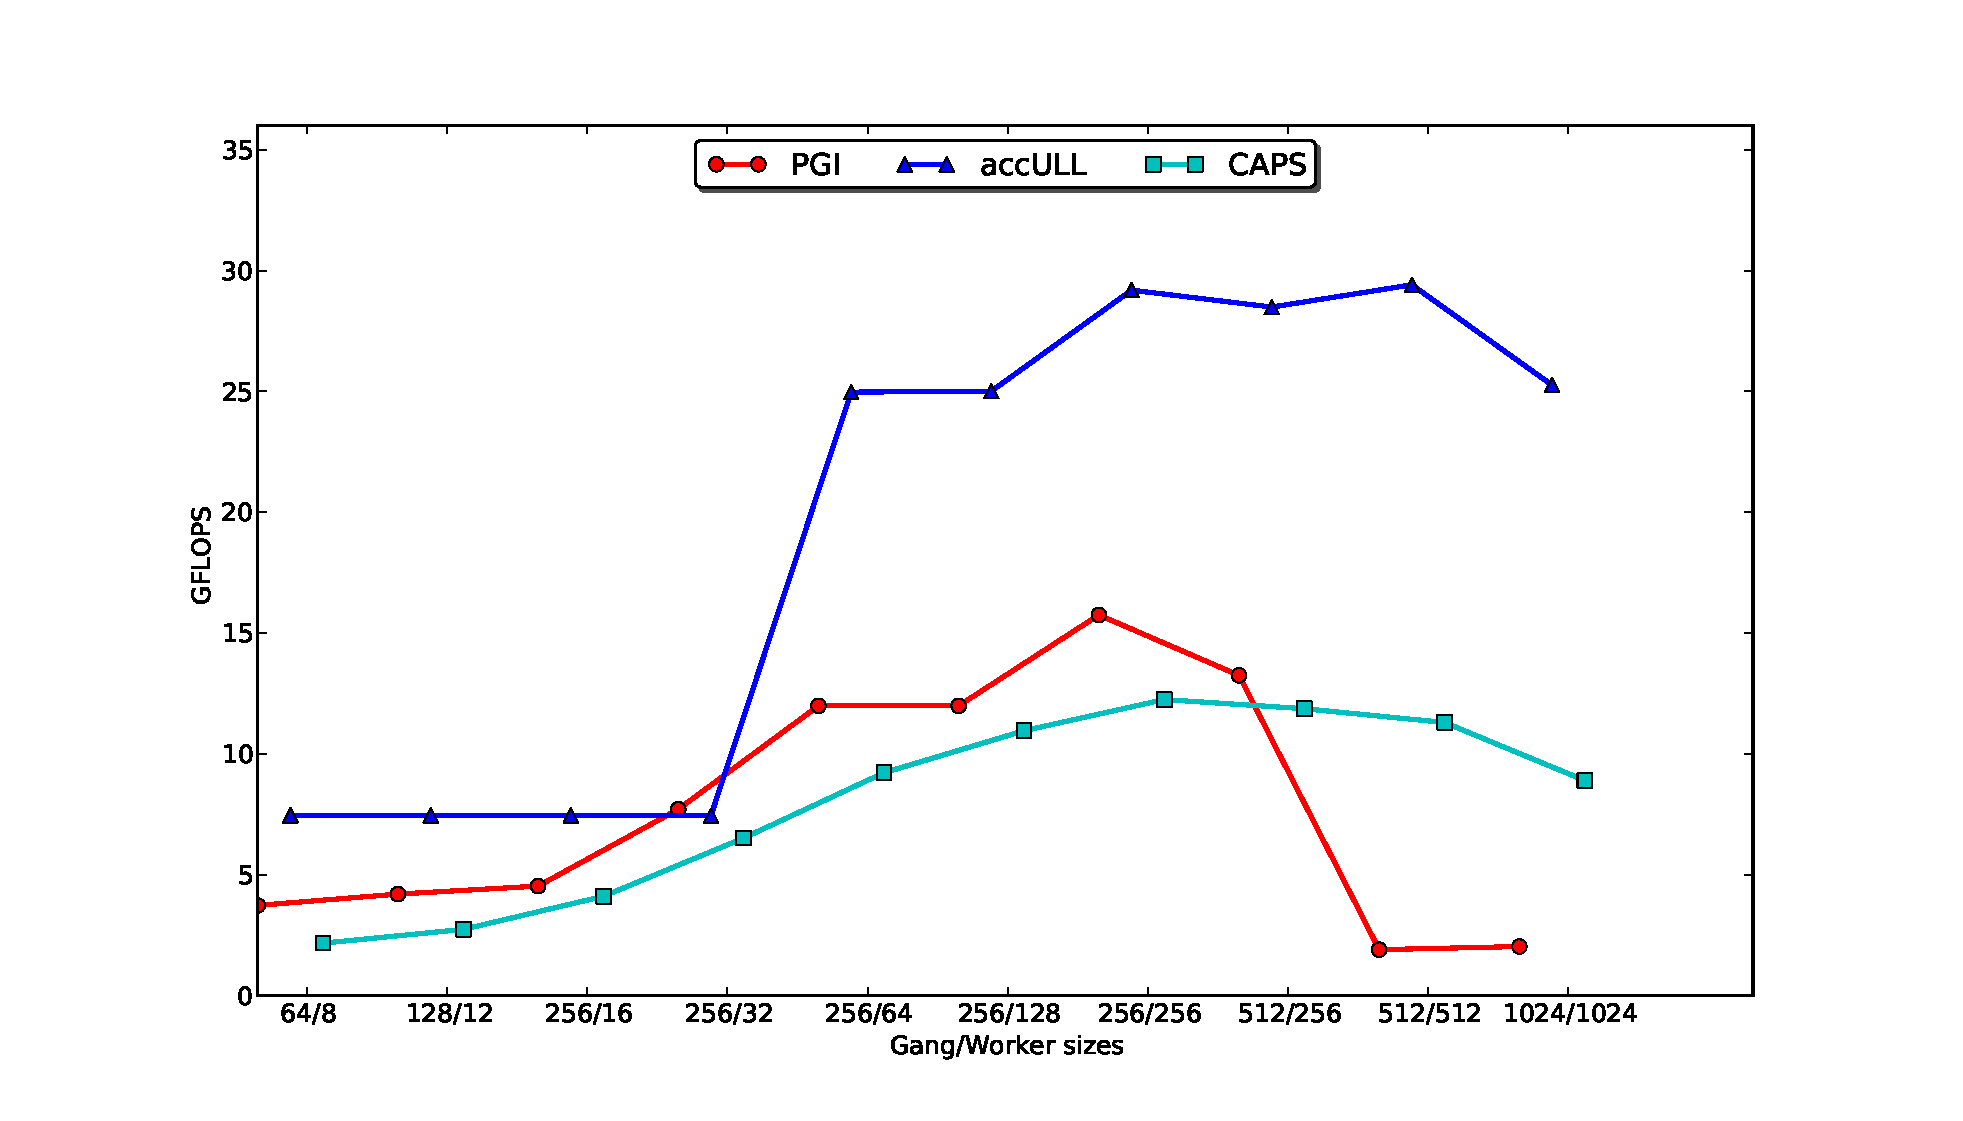
\includegraphics[width=\linewidth]{FIGURES/gemm_flops_varying}
   \caption{Rendimiento de un código \ac{MxM} con distintos valores para un mismo entorno de ejecución.}
   \label{fig:gemm_gangworker}
\end{figure}
%%%%%%%%%%%%%%%%%%%%%%%%%%%%%%%%%%%%%%%%%%%%%%%%%%%%%%%%%%%%%%%%%%%%%%%%%%%%%%%%%%%%%%%%%%


\section{\epcc{} \OpenACC{} \benchmark{} suite}
\label{sec:epccBS}

La suite del \epcc{} \OpenACC{} \benchmark{} \cite{URL::ACCepccB}
publicada en abril de 2013 por N. Johnson y A. Jackson, 
se compone de una serie de operaciones de bajo nivel diseñadas para
verificar el rendimiento potencial de los compiladores y el hardware, además de  
un conjunto de operaciones críticas que simulan aquellas encontradas en los códigos
científicos más frecuentes. 
Esta \textit{suite} está diseñada para ser usada tanto por programadores de aplicaciones 
como por aquellos administradores de sistemas que deseen medir el rendimiento de distintas 
aplicaciones en sus propios equipos informáticos. Usando para ello sus compiladores
y así poder evaluarlos frente a otros sistemas.

La suite la componen 5046 líneas de código de las cuales 140 líneas se corresponden a
etiquetas del tipo \texttt{\#pragma}. Está dividida en varios niveles de complejidad 
creciente. Un primer nivel \textit{level0} formado por códigos simples que verifican 
el correcto funcionamiento de cláusulas como \texttt{copyin}, \texttt{copyout}, etc. y 
pequeñas regiones 
de tipo \texttt{parallel} y \texttt{kernels} con bucles 1D. El segundo nivel, algo más
complejo, contiene códigos con regiones de bucles 2D, reducciones simples, así como
reducciones en kernels 2D. Por último, la suite de \benchmark{}s del \epcc{} se completa 
con el nivel 2, formado por tres códigos de aplicaciones reales habituales en 
diferentes disciplinas científicas.

%%%%%%%%%%%%%%%%%%%% Code  %%%%%%%%%%%%%%%%%%%%%%%%%%%%%%%%%%%
\begin{lstlisting}[caption={Test ATAX del level1},label=code:epcc:atax]
#pragma acc data copyin(A[0:n*n], x[0:n]), create(tmp[0:n])
{
#pragma acc parallel loop private(tmpscalar)
    for (i = 0; i < n; i++){
      tmpscalar = 0;
#pragma acc loop reduction(+:tmpscalar)
      for (j = 0; j < n; j++){
        tmpscalar += A[i*n+j] * x[j];
      }
      tmp[i] = tmpscalar;
    }
    ...
}
\end{lstlisting}
%%%%%%%%%%%%%%%%%%%%%%%%%%%%%%%%%%%%%%%%%%%%%%%%%%%%%%%%%%%%%%

Es importante destacar las reducciones en kernels 2D como 
la mostrada en el Listado \ref{code:epcc:atax} correspondiente al test ATAX. 
El test ATAX, como algunos 
otros del \textit{level1} alberga una región \texttt{parallel} 2D en la que al segundo 
bucle se le aplica una reducción (línea 6) de una variable que es privada al primer bucle 
(línea 3). Esta es una región para la que no es posible distribuir completamente el 
espacio de iteraciones en dos dimensiones como se explicó en la Sección 
\ref{subsec:ecuations}. Esto se debe a que no es posible garantizar la sincronización
entre bloques de \thread{}s, y por lo tanto la variable privada de reducción no asignará
correctamente el resultado real al vector \texttt{tmp}. Como solución provisional,
en \accULL{} se ha optado por evitar distribuir las iteraciones del segundo bucle, 
ejecutando secuencialmente sus iteraciones en cada \thread{} de \gpu{}. La versión 
evaluada de \CAPS{} no es 
capaz de compilar y ejecutar correctamente este tipo de códigos. Se tomará para la 
comparativa la versión de \PGI{} que sí que lo logra.


%%%%%%%%%%%%%%%%%%%%% Table %%%%%%%%%%%%%%%%%%%%%%%%%%%%%%%%%
\begin{table}[htb]
\caption{Tiempos de compilación de los ficheros que componen el \benchmark{}}
\label{table:epccBS:compilation}
\newcommand{\m}{\hphantom{$-$}}
%\newcommand{\cc}[1]{\multicolumn{1}{c}{#1}}
\renewcommand{\tabcolsep}{4pt} % enlarge column spacing
\renewcommand{\arraystretch}{1.2} % enlarge line spacing
\centering
\begin{tabular}{@{}ccccccc}
\hline 
       & Fichero  & Nº de Líneas & Nº de Pragmas &  PGI & CAPS HMPP    & \accULL{} \\ \hline
%\multirow{1}{*}{HS}  
      &  common.c    & 218 & 2 &  0m 0.41s  &  0m24.362s  &  0m 7.21s   \\ \hline
      &  main.c      & 189 & 2 &  0m 3.39s  &  0m32.869s  &  0m 23.612s  \\ \hline
      &  level0.c    & 767 & 45 &  1m 9.67s  &  3m47.581s  &  7m 18.67s  \\ \hline
      &  level1.c    & 1507 & 70 &  1m 22.50s &  2m50.224s  &  20m 48.98s \\ \hline
      &  27stencil.c & 246 & 8 &  0m 6.44s  &  0m42.000s  &  0m 59.05s  \\ \hline
      &  le\_core.c   & 906 & 6 &  0m 7.89s  &  0m44.579s  &  6m 16.00s  \\ \hline
      &  himeno.c    & 279 & 4 &  0m 6.48s  &  0m43.460s  &  0m 51.75s  \\ \hline
      &  Total        & 4112 & 137 &  2m 54.57s &  9m51.493s  &  36m 46.43s \\ \hline
\end{tabular}\\[2pt]
\end{table}
%%%%%%%%%%%%%%%%%%%%%%%%%%%%%%%%%%%%%%%%%%%%%%%%%%%%%%%%%%%%%%

La Tabla \ref{table:epccBS:compilation} muestra el tiempo de compilación de la suite,
con los compiladores evaluados. Destaca el buen rendimiento del compilador de \PGI{}.
En el caso de \accULL{}, su relativa falta de velocidad en el tiempo de compilación
de algunos códigos, es debida en parte a una creciente \acf{TS} que gestiona los símbolos
mediante listas. Haciendo que la búsqueda en la misma sea ineficiente. 
Entre los trabajos futuros se encuentra mejorar la \ac{TS} permitiendo una búsqueda 
mediante funciones de dispersión.
%, también conocidas como funciones \textit{hash}. 
Otro aspecto a evitar con el fin de mejorar los tiempos de compilación, es la
reiterada sucesión de ciclos de parseo y volcado del AST a código fuente, en concreto
en la clase \class{Outliner} de la que hacen uso los diferentes mutadores del \backend{}
de \package{Frangollo}.


%%%%%%%%%%%%%%%%%%%%%%%%%%%%%%%%%%%%% Figure %%%%%%%%%%%%%%%%%%%%%%%%%%%%%%%%%%%%%%%%%%%%%
\begin{figure}[!tbh]
   \centering
   \includegraphics[width=\linewidth]{resultados/epcc_acel_l0}
   \caption{Comparativa de \benchmark{}s del \textit{level0} respecto a \PGI{}}
   \label{fig:epcc_acel_level0}
\end{figure}
%%%%%%%%%%%%%%%%%%%%%%%%%%%%%%%%%%%%%%%%%%%%%%%%%%%%%%%%%%%%%%%%%%%%%%%%%%%%%%%%%%%%%%%%%%

En los tests evaluados se ha tomado un tamaño de problema 1048576.
En las Figuras \ref{fig:epcc_acel_level0}, \ref{fig:epcc_acel_level1} y 
\ref{fig:epcc_acel_level2} se puede apreciar una comparativa de los 
compiladores evaluados en la 
que se mide la aceleración respecto a \PGI{} para algunos tests destacables del 
\textit{level0}, \textit{level1} y aquellos correspondientes al nivel 2. 
A continuación se describen algunos tests que se han mostrado significativos para la 
comparativa de rendimientos entre los compiladores evaluados. 
% VALORES NEGATIVOS: VER los TEST. Por ejemplo en las reducciones indican que las reductions tandan más que el bucle sin etiquetar la reducción ( con el consiguiente resultado incorrecto)
%Para otros tests, por la naturaleza de los códigos que en muchos casos omiten devolver 
%datos, se sospecha que los compiladores han evitado descargar la región o simplemente han 
%descartado ejecutar el código en el dispositivo. 

\subsection{Nivel 0}
\label{subsec:level0}

Los cuatro primeros test miden el tiempo dedicado a las transferencias
de variables hacia y desde el dispositivo. 
Aquí \accULL{} destaca sobre el resto. 
En los test \textit{Kernels\_If} y \textit{Parallel\_If} se mide el \textit{overhead} que 
se agrega a una 
región \texttt{kernels} o \texttt{parallel}, respectivamente, que ha sido etiquetada con 
la cláusula \texttt{if(0)} para su ejecución en CPU. 
En este caso, con la región \texttt{kernels} los tiempos de \CAPS{} y 
\accULL{} son despreciables respecto a \PGI{}. 
Con la región \texttt{parallel},
\accULL{} da un resultado inferior respecto a \PGI{}. Esto se debe a que el registro 
de variables que han de ser transferidas se realiza independientemente de si se va 
ejecutar un kernel en CPU o en el dispositivo.
El test \textit{Update\_Host} mide el tiempo empleado en actualizar una variable en CPU 
después de ser asignada en \GPU{} mediante una región \texttt{kernels}, repetida después 
de la actualización.
En este test, \accULL{} tiene un comportamiento similar a \CAPS{}. \PGI{} podría estar 
omitiendo la ejecución del segundo kernel al realizar un análisis ulterior.
En el test \textit{Kernels\_Invocation} se mide el tiempo correspondiente a 
la invocación de los kernels.
Aquí, el análisis de variables que realiza \accULL{} y la forma en que el test trata de 
medir la invocación puede estar dando mejores resultados para \PGI{}. % <- CONFIRMAR !
% Se mide el tiempo de la ejecución de dos kernels por separado que han de ser ejecutados 
% en serie, al % depender el uno del otro, y posteriormente se substrae el tiempo de 
% ejecución de un kernel combinado. % O eso entiendo. Si es así habría que revisarlo
El último test evaluado, el test \textit{Parallel\_Invocation}, trata de medir la 
invocación de las 
regiones \texttt{parallel} siguiendo el mismo principio descrito para el test 
\textit{Kernels\_Invocation}. En ambos casos los resultados son similares.
% Si el anterior está mal este también !! Parece un copia y pega. % CONFIRMAR !

\subsection{Nivel 1}

%%%%%%%%%%%%%%%%%%%%%%%%%%%%%%%%%%%%% Figure %%%%%%%%%%%%%%%%%%%%%%%%%%%%%%%%%%%%%%%%%%%%%
\begin{figure}[h]
   \centering
   \includegraphics[width=\linewidth]{resultados/epcc_acel_l1}
   \caption{Comparativa de \benchmark{}s del \textit{level1} respecto a \PGI{}}
   \label{fig:epcc_acel_level1}
\end{figure}
%%%%%%%%%%%%%%%%%%%%%%%%%%%%%%%%%%%%%%%%%%%%%%%%%%%%%%%%%%%%%%%%%%%%%%%%%%%%%%%%%%%%%%%%%%

En la Figura \ref{fig:epcc_acel_level1} se presentan algunos resultados de la comparativa
del \textit{level1}. \accULL{} destaca en el test \textit{2MM}, que etiqueta una región 
\texttt{parallel} con tres bucles aplicando una reducción privada al tercero. En la 
práctica
se trata de un código similar al estudiado en el Listado \ref{code:mxm:opt1} puesto que
reduce las operaciones del tercer bucle en una variable privada que en \GPU{} se gestiona
mediante registros.
El test \textit{3MM}, similar a \textit{2MM}, emplea regiones \texttt{parallel} con 
accesos a memoria 
global, para las que \accULL{}-0.3alpha aún no aplica las optimizaciones explicadas en el 
Listado \ref{code:mxm:opt1}. % CONFIRMAR !
Se espera que cuando esta optimización se aplique se obtenga un resultado similar al
obtenido con el test \textit{2MM}.
Los tests \textit{ATAX}, \textit{BICG}, \textit{MVT}, y \textit{GESUMMV} se presentan con 
regiones \texttt{parallel} 2D con 
reducciones privadas en el segundo bucle, del tipo mostrado en el Listado 
\ref{code:epcc:atax}. Como se comentó al inicio de la presente Sección \ref{sec:epccBS},
este es un caso para el que \accULL{} aún puede aplicar algunas mejoras. Cabe destacar que 
con la versión evaluada del compilador de \CAPS{}, estos tests no se han podido compilar. 
Los tests \textit{SYRK} y \textit{COV}, que implementan regiones \texttt{parallel} 2D se 
comportan bien con \accULL{}. El motivo es que en este test hay tantos
\thread{}s disponibles - el valor aplicado en \accULL{}-0.3alpha por defecto es de 16x16 a 
cada bucle - suficientes como para que las ecuaciones de distribución de bucles (véase 
Sección \ref{subsec:ecuations}) hagan su trabajo para las $N^2 = 1048576^2$ iteraciones. 
Esto se refleja en el buen resultado de \accULL{} respecto a \PGI{}. 
En el test \textit{GEMM} se emplea una región \texttt{kernels} 2D para la que \accULL{} 
aún no aplica las ecuaciones de distribución de iteraciones mencionadas. Por lo que queda 
margen para mejorar estos resultados. 
% XXX
%Los tests 2DCONV y 3DCONV alojan regiones \texttt{kernels 
%loop independent}, y sus resultados aún han de ser estudiados. % CONFIRMAR !

%%%%%%%%%%%%%%%%%%%%%%%%%%%%%%%%%%%%% Figure %%%%%%%%%%%%%%%%%%%%%%%%%%%%%%%%%%%%%%%%%%%%%
\begin{figure}[!tbh]
   \centering
   \includegraphics[width=0.9\linewidth]{resultados/epcc_acel_l2}
   \caption{Comparativa de \benchmark{}s del \textit{level2} respecto a \PGI{}}
   \label{fig:epcc_acel_level2}
\end{figure}
%%%%%%%%%%%%%%%%%%%%%%%%%%%%%%%%%%%%%%%%%%%%%%%%%%%%%%%%%%%%%%%%%%%%%%%%%%%%%%%%%%%%%%%%%%

\subsection{Nivel 2}
En la Figura \ref{fig:epcc_acel_level2} se muestran los resultados de la ejecución
respecto al tiempo de \PGI{} con los compiladores evaluados. Estos son tests 
basados en programas científicos reales con una complejidad considerable.
El núcleo pesado de 27S está compuesto de dos regiones \texttt{parallel} 3D, que
\accULL{} convierte en kernels 2D con la consiguiente pérdida de rendimiento.
LE2D contiene dos regiones 2D, que son una región \texttt{kernels} y otra 
\texttt{parallel}. Ambas etiquetadas con cláusulas \texttt{present} que \accULL{} 
gestiona mediante ámbitos adecuadamente. 
LE2D repite la llamada a estas regiones de manera reiterada. Repitiendo el proceso
400 veces. Se estima que el bajo rendimiento en \accULL{} se debe a el \textit{overhead}
de la invocación de las regiones, tal como se pudo apreciar en la Sección 
\ref{subsec:level0} con los tests \textit{Kernels\_Invocation} y \textit{Parallel\_Invocation}. % CONFIRMAR!

En muchos casos las regiones \texttt{parallel} pueden estar distribuyendo las iteraciones 
en una pequeña cantidad de \thread{}s - en \accULL{}-0.3alpha si no se indica nada mediante 
las cláusulas \gang{} y \worker{} por defecto se asignan 16 bloques de 16 \thread{}s cada 
uno. Pese al bajo rendimiento de algunos de estos resultados, el mayor logro estriba en 
lograr que \accULL{} compile y ejecute una serie de códigos escritos en \OpenACC{} por un 
tercero autorizado, en este caso investigadores miembros del \epcc{}. Como línea de 
trabajo futuro se tratará de analizar y estudiar cómo mejorar el rendimiento de estos 
códigos, que sin duda alguna han servido para evaluar cualitativamente el framework
de compilación que compone \accULL{}.
